\section{Initial Experiments}\label{sec:initial_experiments}

In this section, some initial experiments will be introduced and analyzed. This will be done to address some of our issues with E3. Since there is no documentation, we conduct these experiments in an attempt to get more insight into how E3 works. This will not be done for Intel power Gadget, RAPL and LHM as no issues has been observed when creating the framework. Secondly, the configuration introduced in \cref{subsec:sql} needs some values for what ranges of battery percentages and temperatures are ideal for the experiment to run in.

\subsection{E3 Experiments}

The following experiments with E3 address some of the discoveries made in the initial testing, which contradicts the statements in the available sources\cite[]{E3Doc,E3Video,E3WinHec}. 

This experiment was conducted based on observations where there were deviations from the expected output in the log file according to the sources and the actual output. In the output log file for E3, each row represents the measurement of one application in a given state. It is claimed that an application needs to run for $1-5$ minutes before it is added to the file. Based on observations this is not true, as the lowest measurements were observed to be as low as  $0$ and $1.554$ seconds. The highest value found in the test is $902$ minutes, which also does not match the claim. Another aspect is that E3 counts the same application as different measurements depending on its status.
Example \texttt{App.Status=Focus}, \texttt{App.Status=Visible}, \texttt{App.Status=Minimized} and \texttt{App.Status=NotUnique} will all be counted as different measurements in E3. Where \texttt{App.Status=Focus} is when the application is in focus. \texttt{App.Status=Visible} is when the application is not in focus, but still visible on the screen. \texttt{App.Status=Minimized} is when the application is minimized. \texttt{App.Status=NotUnique} are background processes which do not have a user interface. This has been concluded by looking at the processes with this status and the frequency of their repetition over a period. 
Because of the uncertainty about how E3 functions it was deemed necessary to conduct some further experiments to determine when a process is included in the measurements and when it is not. To carry out these experiments different scenarios were formulated, which will be covered now.

% \begin{itemize}
%     \item Order of measurement
%     \begin{itemize}
%         \item Scenario 1: A process is started before the measurements and ended after the measurements
%         \item Scenario 2: A process is started during the measurements and ended after the measurements
%         \item Scenario 3: A process is started before the measurements and ended during the measurements
%     \end{itemize}
%     \item State Change
%     \begin{itemize}
%         \item Scenario 4: Several process "state" are swapped between with increasing intervals
%         \item Scenario 5: Several process "state" are swapped between with a fixed interval
%         \item Scenario 6: Change The "state" of a single process during measurements
%     \end{itemize}
%     \item Instances
%     \begin{itemize}
%         \item Scenario 7: A process opened and restarted several times during the measurements
%         \item Scenario 8: Several instances of the same application
%     \end{itemize}
%     \item Measurement resolution
%     \begin{itemize}
%         \item Scenario 9: Taking several measurements with different durations
%     \end{itemize}
% \end{itemize}

\paragraph{Order of measurement}

\begin{itemize}
    \item Scenario 1: A process is started before the measurements and ended after the measurements
    \item Scenario 2: A process is started during the measurements and ended after the measurements
    \item Scenario 3: A process is started before the measurements and ended during the measurements
\end{itemize}

\paragraph {Expectations}
The first three scenarios are designed to see when measurements are recorded by E3. The initial expectation is that E3 uses the start and exit timestamp for the measured process. Because of this, expectations are that scenarios 1 and 2 would not record a process but that scenario 3 would.

\paragraph{Findings}
Scenarios 1 and 2 were both contrary to our expectations, where scenario 1 resulted in several measurements of the process, and similar results were obtained from scenario 2. In scenario 3, the process is not found, which is also contrary to our expectations. These results point to E3 instead of using the start and end times instead take several snapshots of the process over some time. Exactly how frequent these snapshots are will be tested later. 

\paragraph{State Change}

\begin{itemize}
    \item Scenario 4: Several process "states" are swapped between with increasing intervals
    \item Scenario 5: Several process "states" are swapped between with a fixed interval
    \item Scenario 6: Change The "state" of a single process during measurements
\end{itemize}

\paragraph{Expectations}
Scenarios 4 and 5 are meant to see how E3 handles changes in the process state during the measurements. Scenario 4 attempts to see how granular a new state is measured. While scenario 5 uses the lowest measurement found in scenario 4 to check for consistency. The expectation is that each state change will be measured, until a certain threshold where the change will no longer be registered as the swapping is more frequent than E3's sampling. Scenario 6 is designed to test something similar to scenario 4 but instead uses the same process to see how that changes the results.
\paragraph{Findings}
For scenarios 4 and 5, swapping between the states is only recorded at the first occurrence, and then the results for further state changes are aggregated together. The speed of the change does not hinder E3's measurements contrary to our expectations and does not create a measurement for each state change. Scenario 6 had the same results as 4 and 5 but provided some insight. Each application instance has the same id in E3 and cannot be differentiated based on it, but the execution time for each instance is carried over from state to state, so using this, two identical processes, can be identified since the time reported by E3 is the total execution at the time of collection.

\paragraph{Instances}

\begin{itemize}
    \item Scenario 7: A process opened and restarted several times during the measurements
    \item Scenario 8: Several instances of the same application
\end{itemize}

\paragraph{Expectations}
Scenario 7 is designed to see how E3 looks at multiple starts and shutdowns during measurements. The expectation is that each instance will be a separate measurement. Scenario 8 is designed to see how E3 handles multiple concurrent instances of the process with the same process id the expectation here is that the measurements will be merged into one big measurement. 
\paragraph{Findings}
In scenario 7 a process opening and closing within 1 second seem to not always get picked up by E3, but the instances that do get picked up seem to be aggregates of the instances recorded. This could indicate that E3 might not be able to tell the difference between the instances if they are opened and closed fast enough but still knows that they did execute. In scenario 8 several instances of the same application are not immediately identifiable in E3 since they have the same id, but by looking at the execution time in each recording the different instances can be identified.

\paragraph{Measurement resolution}

\begin{itemize}
    \item Scenario 9: Taking several measurements with different durations
\end{itemize}

\paragraph{Expectations}
Scenario 9 is designed to test if E3 uses a per-application sampling rate or if it has a global sampling rate and exactly how frequent it is. The expectation for Scenario 9 is that measurements with durations less than $1$ minute will be inconsistent as we expect a global sampling around once every minute.

\paragraph{Findings}
Scenario 9 confirmed our understanding of E3 as it showed that a new snapshot was taken exactly at the start of a minute.

\paragraph {Recommended usage}
From the experiments, several aspects of E3 has been uncovered, and an understanding of its inner working has become deep enough to utilize for further experimentation. The important aspects that were learned are summarized below:

%% 

\begin{itemize}
    \item E3 takes the measurements in snapshots, which contain every active process on the system
    \item If a program is active during the snapshot it will be included, unaffected by process start, but it has to be active at the end of the snapshot
    \item Change state will only be recorded once every snapshot
    \item The separate measures of the same instance in different states are linked
    \item Each snapshot is taken at the start of every minute
\end{itemize} 

Taking these discoveries into account a process for recommended usage can be created. Our process for using E3 is the following: Await the start of a new snapshot and then execute the program repeatedly until another snapshot is taken. The energy for the test case is then calculated by going through the measurement experiment id and summing each of their energy usages to get the dynamic energy usage for the whole test case. There must be some time between the snapshot for the next measurement to not include the same process twice, our findings suggest that $2$ minutes is adequate for isolating the measurements.    
\subsection{Experiment Representation}\label[subsec]{subsec:exp_rep}

After the introduction to the framework in \cref{subsec:framework}, the format of the data in \cref{subsec:sql}, the different DUTs, test cases and measuring instruments in \cref{sec:hardware}, \cref{subsec:test_cases}, \cref{sec:measuring_instruments} respectively, the experiments can now be introduced. This will be done in the context of the different terms related to the experiments found in \cref{tab:TerminologyAlert}.

\paragraph{}
When running the experiments, it will be done based on different experiment configurations. These configurations will be different DUTs, test cases and measuring instruments. Here the same computer running either Windows or Linux will count as different DUTs. In the framework, a test case will run for a minimum period of time, before switching to the next configuration, and based on what was found in \cref{sec:E3Experiments}, this period will be one minute, since that is required in order to use E3. In this period of one minute, the total energy consumption will be captured, in addition to how many times the test case was executed, which means an average energy consumption per test case run can be calculated. After this one minute of execution, there is an optional cooldown period, which is required for E3. However since E3 is not used in the initial experiment a cooldown period is not used. This was chosen as no argument was found as to why it should be used or what the value should be. However, there is an indirect cooldown period of about $\approx30$ seconds as the measurements are sent to the database and the setup phases is entered to ensure background processes and WiFi is turned off.

During one minute, the test case will execute $n$ times, resulting in $n$ samples, according to \cref{tab:TerminologyAlert}. When the test case has been executed for one minute, this will be called a measurement. When the same configuration has been executed multiple times, it is a test case measurement according to \cref{tab:TerminologyAlert}.

\paragraph*{}
As was introduced in \cref{subsec:cock}, Cochran's formula will be used to calculate how many measurements are required, in order for the results to be within some pre-defined standard deviation. Before this value is chosen, an arbitrary value of 120 is used. Meaning that we run for one minute a 120 times. 
%In addition to this, a value is also needed for how many measurements $m$ should be made for each measuring instrument between restarts. On start up, one test case is chosen to be executed until the next restart. For this test case, each measuring instrument needs to make $m$ measurement before the DUT restarts. This is done to ensure there will be multiple measurements where each test case is run with each measuring instrument for the $1 \dots m$'th time after a restart. Here $m=30$ was chosen, as this would result in each configuration having four measurement, where it was the first measuring instrument on a specific test case to run.
If based on Cochran's formula the values are not deemed sufficient, additional experiments will be executed.

 %for each $m$ times a test case is executed after a restart.

%For this test case, we need to take $m$ measurements with each instrument before the device under test (DUT) is restarted. This is to ensure that there are multiple measurements for each run after a restart. We chose $m=30$ so that each run after a restart would have four measurements. If the sample size is not large enough according to Cochran's formula, we will conduct additional experiments.

\paragraph*{}
In addition to this, R3 validation\cite[]{Bokhari2020r3} will also be utilized in an adapted manner. The idea from the original article was to compare different implementations of the same test case, to see which version performed best. The idea was to switch between which implementation was the first to run after a restart, to make the comparison fairer. In our work, it is a bit different, where different measuring instruments will be compared. When running the experiment, with three measuring instruments $A, B$ and $C$ and test cast $T$ and DUT $D$, $D$ will execute $T$ $m$ times in a row. The first time $A$ will measure the energy consumption, then $B$ etc. When $D$ has reached a state where it needs to restart (after $m$ measurements), it will save which measuring instrument was used first. When $D$ has restarted, it will again execute $T$, but this time $B$ will measure first, then $C$ and so on. This will continue until the measuring instruments have 120 measurements each.\todo{I have moved part about m to here instead of cochrans} Therefore, a value is also needed for how many measurements $m$ should be made for each measuring instrument between restarts. This is done to ensure there will be multiple measurements where a test case is run with a measuring instrument for the first time after a restart. Here $m=30$ was chosen, as this would result in each configuration having four measurement, where it was the first measuring instrument on a specific test case to run, which is important to avoid measurements for specific configurations being affected by variables in changing system states.

\subsection{Expected Energy Consumption} \label[subsec]{subsec:expec_energy_consumption}

In this section, the expected energy consumption of the different components within the DUTs will be covered. The values and calculations will be covered, in addition to the rationale behind them. This will be achieved by looking at the expected range of energy consumption of each component individually, this will then provide a lower and upper limit for the consumption of the DUT.

When referring to the energy consumption of computer components, a common term is Thermal Design Power (TDP). In the work by Hennessy\cite{hennessy2011computer}, TDP is defined as a representation of the average power a processor will draw, when all cores are active and under a high complexity workload. While under peak workload the processor can reach around $1.5$ times more than its TDP. The lower power limit of a CPU is disputed, but it is approximated To be around $10-25$W for most modern CPU's\cite{CPUPowerCum}.

\paragraph{Workstation} The first DUT is the workstations, and the energy consumption for the different components can be seen in \cref{tab:WorkstationEstEnergCon}.

\begin{table}[ht]
    \centering
    \begin{tabular}{||c | c | c | c | c | c ||}
    \hline
    % \multicolumn{5}{l}{Workstation} \\
    \multicolumn{6}{||c||}{\textbf{Workstation}}           \\
     & \textbf{RAM}\cite{buildComputerRAM} & \textbf{CPU}\cite{IntelCPUi7} & \textbf{SSD}\cite{tomshardwareSSD} & \textbf{Motherboard}\cite{CPUPowerCum} & \textbf{Fans}\\[0.5ex] \hline\hline
    Minimum consumption & $2 * 1.5$W & $10$W   & $0.2$W & $15$W & \\
    Average consumption & $2 * 2.25$W & $65$W   & $6$W & $37.5$W & \\
    Maximum consumption & $2 * 3$W & $97.5$W & $9$W &  $60$W & $2 * 2.4$W \\ \hline
    \end{tabular}
    \caption{The energy consumption for the different components in the workstation}
    \label{tab:WorkstationEstEnergCon}    
\end{table}


\todo{Add second SSD}
The power supply does not have a specific energy consumption but instead has an energy efficiency rating. The energy efficiency rating represents how much of the energy going into the power supply, is used by the system. The power supply used in the workstation has an 80-Plus Gold certification, representing an efficiency of $90\%$ at a load of 20\%, an efficiency of $92\%$ at a load of 50\% and an efficiency of $89\%$ at a load of 100\%. This is highly relevant for the clamp measurements as they are measured before going into the power supply and will thus be around 8-11\% higher that the actual system consumption.

Using these values lower and upper bounds for the expected energy consumption can be created for the DUTs.

\paragraph{Software measuring instruments}: The different software approaches measure the CPU and ram individually so the Min and Max values for these components are the values the measurements should be between. Given the test cases will not put the DUT under a significant load, the measurements would be expected to be close to the following:

\begin{gather*}
    CPU: 10W < x < 65W \\
    Ram: 1.5W < y < 2.25W \\
    \text{Where $x$ and $y$ represent the measured energy consumption of the CPU and Ram respectively.}
\end{gather*}

\paragraph{Clamp measurements:} The clamp measurements include the energy consumption of the entire system. To calculate the lower and upper limits to the energy consumption, the values found in \cref{tab:WorkstationEstEnergCon} are summarized. Based on our observations, the CPU never utilizes more than $40\%$. Because of this, and as there is no GPU in the DUT, the efficiency of the power supply is set to the minimum efficiency for the calculations. The lower bound is thus calculated based on:

\begin{equation}
    Min = {MinCPU, MinBoard, MinRam, AvgSSD, CPUFan, CaseFan}
\end{equation}

Based in $Min$, the $LowerCase$ can be calculated, representing the minimum energy consumption of the DUT. This is calculated as:

\begin{equation}
    LowerCase = \left ( \sum_{m \in Min} m \right ) * \left (1 + \left ( \frac{1}{MinEff} \right ) \right ) = 35.75W
\end{equation}

A thing to note here, is how $avgSSD$ was used instead of $minSSD$. This decision is based on observations, where the SSD is used by the OS all the time. Next up, the average case can be calculated. Here, the equation is the same, but the values change. They are as following:

\begin{eqnarray}
    Avg = {AvgCPU, AvgBoard, AvgRam, AvgSSD, CPUFan, CaseFan}
\end{eqnarray}

And $AverageCase$ is as following:

\begin{equation}
    AverageCase = \left ( \sum_{a \in Avg} a \right ) * \left (1 + \left ( \frac{1}{MinEff} \right ) \right ) = 119.6W
\end{equation}

The measurements from the clamp are expected to be between the $LowerCase$ and $AverageCase$.

\paragraph{Surface Book:} As the Surface Book is a laptop and is running on a battery, the clamp measurement setup will not be used on this DUT. Thus only the CPU and RAM will be subject to the measurements. The energy consumption of the components of this DUT can be seen in \cref*{tab:bookjuanEstEnergCon}

\begin{gather*}
    CPU: 7.5W < x < 14W \\
    Ram: 2W < y < 2.5W \\
    \text{Where $x$ and $y$ represent the measured energy consumption of the CPU and Ram respectively.}
\end{gather*}


\begin{table}[ht]
    \centering
    \begin{tabular}{|| c | c | c ||}
    \hline
    % \multicolumn{5}{l}{Surface Book 1} \\
    \multicolumn{3}{||c||}{\textbf{Surface Book}}           \\
     & \textbf{RAM}\cite{buildComputerRAM} & \textbf{CPU}   \cite{NotebookCPU} \\ [0.5ex] \hline\hline
    Minimum consumption & $2$W& $7.5$W \\ 
    Average consumption & $2.5$W& $14$W \\ 
    Maximum consumption & $3$W & $21$W \\ \hline
    \end{tabular}
    \caption{The energy consumption for the different components in the Surface Book}
    \label{tab:bookjuanEstEnergCon}    
\end{table}

\paragraph{Surface Pro 4} The Surface Pro 4 is also a laptop and is hardware wise similar to the Surface book. They are similar in terms of the RAM, and the CPU is from the same generation, but CPU in the Surface Pro 4 is slightly better with a higher turbo clock speed and bigger L3 cache. The energy consumption for the Surface Pro 4 can be seen in \cref{tab:proQuadroEstEnergCon}, and the upper and lower bounds are as follows:

\begin{gather*}
    CPU: 9.5W < x < 15W \\
    Ram: 2W < y < 2.5W \\
    \text{Where $x$ and $y$ represent the measured energy consumption of the CPU and Ram respectively.}
\end{gather*}

\begin{table}[ht]
    \centering
    \begin{tabular}{|| c | c | c ||}
    \hline
    % \multicolumn{5}{l}{Surface Pro 4} \\
    \multicolumn{3}{||c||}{\textbf{Surface Pro 4}}           \\
     & \textbf{RAM}\cite{buildComputerRAM} & \textbf{CPU}\cite{IntelCPUSpec} \\ [0.5ex] \hline\hline
    Minimum consumption & $1.5 * 2$W& $9.5$W \\
    Average consumption & $2.25 * 2$W& $15$W \\
    Maximum consumption & $3 * 2$ & $22.5$W\\ \hline
    \end{tabular}
    \caption{The energy consumption for the different components in the Surface Pro 4}
    \label{tab:proQuadroEstEnergCon}    
\end{table}

These should be considered rough estimates for what the DUTs can consume, values both above and below these estimates might still be valid, but require some further investigation if the deviation is significant.
\subsection{Anomalies Detection}\label[]{subsec:anomalies_detection}

Anomaly detection was found in \cref*{subsec:anomalies} to be an important tool to avoid corrupted results. For this, DBScan was found to be the algorithm of choice in order to find anomalies in the data.

In order to use this algorithm, 

\begin{figure}[h]  
    \centering 
    \begin{subfigure}[b]{0.4\linewidth}
    \begin{tikzpicture}
        \pgfplotsset{%
        width=1.1\linewidth,
        % height=1\textheight
        }
        \begin{axis}[%
        scatter/classes={%
            a={mark=o,draw=black},
            b={mark=o,draw=red}}]
        \addplot[scatter,only marks,%
            scatter src=explicit symbolic]%
        table[meta=label] {
        x y label
        0.01327654701428432 0.30597463760729066 a
        0.013287214504152108 0.3059995922112346 a
        0.0132497346021537 0.30596372124789123 a
        0.013158449009557673 0.30580162704335556 a
        0.01313797768053797 0.30577598940559264 a
        0.013194376966146148 0.30571795237416227 a
        0.01317422646947403 0.3058300898661178 a
        0.013201657630442327 0.30586281213220495 a
        0.013220625039478722 0.3058242782693748 a
        0.013111049404297848 0.3066686419551269 a
        0.01312265426964118 0.30576849611613394 a
        0.013152599919953963 0.3057226231278105 a
        0.013200018666587876 0.3057086112950043 a
        0.013137469913893819 0.3061576279311716 a
        0.013167521215536533 0.3061826119775994 a
        0.013181599932276147 0.3061342090903991 a
        0.013269674132419307 0.3060261109383523 a
        0.01311017363450352 0.30582499541499397 a
        0.013211053243522152 0.3056063205371642 a
        0.013188753232014442 0.30565837911598326 a
        0.01345422403020393 0.30589200454524607 a
        0.013497149786396233 0.30585388220908905 a
        0.013226068012040314 0.3055277046869195 a
        0.013181406587386865 0.30556658420629346 a
        0.01306641583877133 0.30664984368934023 a
        0.013218005320030996 0.3059559243252059 a
        0.013108030686125585 0.30660599003023614 a
        0.013050415923486849 0.30594345007542706 a
        0.01314818663809047 0.306654543039727 a
        0.013309818005141062 0.30682265393009195 a
        0.013297092067359819 0.3068698700847362 a
        0.013184565376598055 0.30549971755868927 a
        0.01343656295037907 0.3061697038317752 a
        0.013401106220029024 0.30616585067319463 a
        0.013433911438417769 0.30610257299325905 a
        0.013294815371253803 0.30570436305862225 a
        0.013092400605551505 0.30589668069667664 a
        0.013271570412161964 0.3058094161037585 a
        0.013313110996657983 0.3057479577077434 a
        0.013496671666510841 0.3058269738249768 a
        0.013444013781810277 0.3057533437235787 a
        0.01337261019607976 0.3068128385975672 a
        0.013093291984656643 0.3059766154598926 a
        0.013157021043144632 0.3060280885988836 a
        0.013391326336925628 0.3057735897109385 a
        0.01324913552760757 0.30616189640751545 a
        0.013346689323381145 0.3060592928700706 a
        0.013236915000708909 0.3051347999349382 a
        0.0131490784675332 0.30625133913540314 a
        0.013403327460909524 0.30627477590086066 a
        0.013571995634517737 0.3058986588398353 a
        0.013518267968393399 0.30572998630018383 a
        0.01316795231659627 0.3060472277167153 a
        0.013350905036135742 0.3056599354372244 a
        0.013246347686254153 0.3066984105899363 a
        0.013276364511579115 0.3066138201208456 a
        0.013299190336140692 0.3055883610596404 a
        0.01348382688818378 0.30624665221272795 a
        0.013264491226657547 0.3067043358758347 a
        0.013215459756840872 0.3051321280261867 a
        0.01327922032662637 0.30545308373742563 a
        0.013482687699285891 0.30554325530734505 a
        0.013294572104089282 0.3062415508225992 a
        0.013340509808413392 0.30632322325182676 a
        0.013414588545749902 0.30589979821039115 a
        0.013582545043481276 0.30589979821039115 a
        0.013135649231639781 0.3064885866429771 a
        0.013044427510689101 0.3064514482322072 a
        0.013390966133024594 0.3055494759987581 a
        0.013335815135352123 0.30692031615865195 a
        0.01342418175669348 0.3068720318578461 a
        0.013217550976775332 0.30658134629821615 a
        0.013173354014287096 0.3050510696681742 a
        0.01369835175249967 0.30627831517080933 a
        0.013614464384301946 0.30634198118021677 a
        0.013627092807553247 0.30623727879774115 a
        0.013141867668741525 0.30529195781079954 a
        0.013485781246519469 0.3056490415213462 a
        0.013320834605748389 0.3051425550624965 a
        0.013179177472184738 0.3064823276544256 a
        0.013065531362449931 0.306236864121452 a
        0.013157375180113808 0.3053960146715436 a
        0.013275402611545174 0.3064056757860351 a
        0.013316138143520681 0.30650736514258 a
        0.013211263419468915 0.306315408126298 a
        0.013795925127810109 0.30622238999357254 a
        0.01348044625275882 0.3054803582332587 a
        0.013786089422695706 0.30694188085754753 a
        0.013372137872438886 0.3066647595792829 a
        0.01380992516526564 0.30632634941369774 a
        0.013313621379928108 0.30544220456095006 a
        0.013584278123237004 0.3063587649910692 a
        0.013060007456381894 0.3055848261327713 a
        0.013651242810114615 0.30646124630534327 a
        0.013480012690027934 0.3053525195957253 a
        0.013897221754789638 0.3069689671570357 a
        0.013068652976625036 0.3063705351902791 a
        0.013522374980954304 0.30732960973936546 a
        0.013406118632536861 0.30726196935109074 a
        0.013247543424122377 0.30529506295896985 a
        0.013871734254857921 0.3078749647408775 a
        0.013375217026535664 0.30650308126681675 a
        0.013954420136811033 0.30780234937010015 a
        0.013492579173059393 0.30658134629821615 a
        0.013515428950389227 0.3053334554036458 a
        0.013155313038019353 0.3068508835150456 a
        0.012992287424136745 0.3056754995213557 a
        0.013477218358724912 0.30716961051188113 a
        0.013902639044753893 0.30609872376008934 a
        0.013903225865023718 0.3068148133004876 a
        0.01373000864252581 0.30701763358154 a
        0.01380632195165261 0.3065652800049025 a
        0.013507313866522477 0.3074271901837977 a
        0.013749929956988928 0.3078086623903357 a
        0.013895329707810858 0.3076757532281205 a
        0.013721992946543811 0.30664671086909884 a
        0.013766372106681574 0.3059418908657252 a
        0.013700977108123838 0.3072187423237534 a
        0.013961186125864153 0.3070804517739493 a
        0.013742963092909751 0.30724232700250265 a
        0.0140643951024605 0.3061400377377735 a
        0.013406279749500588 0.30488994078031834 a
        0.01333807695082713 0.307547285805037 a
        0.013579416927623324 0.30771438823107283 a
        0.013281288750921228 0.30788325136037503 a
        0.013902835127531035 0.30814594497576986 a
        0.01444845749099448 0.30716920888488636 a
        0.013407502190774884 0.3040267810567578 a
        0.01779387677628413 0.32026269319206374 a
        0.020303868317634872 0.3218492486020191 a
        0.01779387677628413 0.32026269319206374 b
        0.020303868317634872 0.3218492486020191 b
            };
        \end{axis}
    \end{tikzpicture}
    \caption{The outliers (red) based on the 4-dist sorted graph} \label{fig:outliers}  
\end{subfigure}
\begin{subfigure}[b]{0.4\linewidth}
    \begin{tikzpicture}
        \pgfplotsset{%
        width=1.1\linewidth,
        % height=1\textheight
        }
        \begin{axis}[%
        scatter/classes={%
            a={mark=o,draw=black},
            b={mark=o,draw=red}}]
        \addplot[scatter,only marks,%
            scatter src=explicit symbolic]%
        table[meta=label] {
        x y label
        0 2.8949479214654294e-05 a
        1 3.179477203046875e-05 a
        2 3.267322064601172e-05 a
        3 3.280798350852557e-05 a
        4 3.280798350852557e-05 a
        5 4.203733493201637e-05 a
        6 4.2699125166050646e-05 a
        7 4.294905342573423e-05 a
        8 4.676111584622105e-05 a
        9 4.843067177105661e-05 a
        10 4.8774191374681006e-05 a
        11 4.9445616498532656e-05 a
        12 4.9445616498532656e-05 a
        13 4.9958989436862796e-05 a
        14 5.0408826155301995e-05 a
        15 5.0408826155301995e-05 a
        16 5.193014842759746e-05 a
        17 5.634406741910958e-05 a
        18 5.6633789754044637e-05 a
        19 5.6633789754044637e-05 a
        20 5.7410217372431694e-05 a
        21 5.7410217372431694e-05 a
        22 5.921367982846027e-05 a
        23 5.921367982846027e-05 a
        24 6.0456090984576906e-05 a
        25 6.145988034834584e-05 a
        26 6.272460722809678e-05 a
        27 6.284972805645797e-05 a
        28 6.300710443137074e-05 a
        29 6.355470081318446e-05 a
        30 6.359467248323007e-05 a
        31 6.694121683315767e-05 a
        32 6.718318238640716e-05 a
        33 7.127585237345829e-05 a
        34 7.127585237345829e-05 a
        35 7.155322529164951e-05 a
        36 7.38556711976285e-05 a
        37 7.41805540625215e-05 a
        38 7.41805540625215e-05 a
        39 7.765820244366868e-05 a
        40 7.784120665026037e-05 a
        41 7.850775711089268e-05 a
        42 7.993973309373286e-05 a
        43 8.191994222015357e-05 a
        44 8.230819546665794e-05 a
        45 8.420232050680483e-05 a
        46 8.426994000106784e-05 a
        47 8.427717433224613e-05 a
        48 8.479177316626968e-05 a
        49 8.527074308148876e-05 a
        50 8.721724394873936e-05 a
        51 8.722066451929488e-05 a
        52 8.804553811338067e-05 a
        53 8.830233135155855e-05 a
        54 8.975832698738875e-05 a
        55 8.975832698738875e-05 a
        56 8.994826250782899e-05 a
        57 9.030466847320144e-05 a
        58 9.129116493983801e-05 a
        59 9.134194523707361e-05 a
        60 9.161579912448281e-05 a
        61 9.193227245685756e-05 a
        62 9.370516727749144e-05 a
        63 9.370516727749144e-05 a
        64 9.447030026752446e-05 a
        65 9.695684147183935e-05 a
        66 9.84919485426008e-05 a
        67 9.84919485426008e-05 a
        68 9.967369188253414e-05 a
        69 0.00010069773319988507 a
        70 0.00010069773319988507 a
        71 0.00010084232469055083 a
        72 0.00010512257877014406 a
        73 0.00010531121163963648 a
        74 0.00010531121163963648 a
        75 0.00010546120599483379 a
        76 0.00010572136596011746 a
        77 0.00010583143723479704 a
        78 0.00010588947949861364 a
        79 0.00010619424500734341 a
        80 0.00010702116161766447 a
        81 0.00010720818806042881 a
        82 0.00010954500810094572 a
        83 0.00010954500810094572 a
        84 0.00011073430522929063 a
        85 0.00011246416770882411 a
        86 0.0001130661635295037 a
        87 0.00011438558850046904 a
        88 0.00011469125335755415 a
        89 0.00012147392693952117 a
        90 0.00012237591171992 a
        91 0.0001224201334093466 a
        92 0.00012276203358687853 a
        93 0.0001248071419298498 a
        94 0.00012783937274188738 a
        95 0.00012853116577443856 a
        96 0.00013370751331335452 a
        97 0.00013450189840040735 a
        98 0.00013450189840040735 a
        99 0.00013535715902440975 a
        100 0.00013868052735234137 a
        101 0.00013946592819106236 a
        102 0.00013970777345427544 a
        103 0.000146505571066363 a
        104 0.00015101069658064682 a
        105 0.00015706270827900125 a
        106 0.00016013706955956582 a
        107 0.0001662494310569234 a
        108 0.0001669486955830121 a
        109 0.00017282103511564564 a
        110 0.0001741512152900111 a
        111 0.0001867419363296455 a
        112 0.00019374828758415263 a
        113 0.00019483919084249817 a
        114 0.00019699221542950795 a
        115 0.00019850109877225447 a
        116 0.00019912614342020588 a
        117 0.0002031933960156964 a
        118 0.0002232952178907816 a
        119 0.00022506654839991077 a
        120 0.000280816704139863 a
        121 0.0002832259109375601 a
        122 0.00028521681835927984 a
        123 0.00029354421334281766 a
        124 0.0003426297800563272 a
        125 0.00034744633170887413 a
        126 0.0005864789735718681 a
        127 0.0010507104872560743 a
        128 0.012726185306264882 a
        129 0.015124607637026024 a
        };
        \draw[gray, dashed] (127,0) -- (127,1);
        \draw[gray, dashed] (0,0.0010507104872560743) -- (129,0.0010507104872560743);
        \end{axis}
        % \draw[gray, thick] (128,-1) -- (128,2);
    \end{tikzpicture}
    \caption{A 4-dist sorted graph} \label{fig:4-dist}  
\end{subfigure}
\caption{An example of how outliers are found for on the workstation for Fasta measured by HardwareMonitor}
\end{figure}



\subsection{Temperature and Battery Experiment}

One thing to consider before running the experiments, is to determine some of the values for the configurations. This includes at what range of temperature and what range of battery percentage the system should be within without a degrading performance. The reason why these ranges are chosen is first of all based on the work by Bokhari et al.\cite*[]{Bokhari2020r3} where experiments were only run when the battery percentage was above a certain limit, as phones cpu will enter power saving mode. Because of this, the hypothesis will be that a similar observation can be made on laptops. Another parameter able to make the DUT underperform is the temperature, as was noted in the work by Lindholt et al.\cite*[]{Lindholt2022}. 

Based on these two parameters, the assumption would be that there is some lower limit on the battery where the CPU is under clocked, and some upper limit for the temperature where the CPU will thermal throttle, resulting in a much worse performance. In order to find these values, a test case will be executed on all DUTs, where the battery will decrease, and the temperature will increase during the experiments. These values will then be plottet for each DUT, where the X-axis will represent the temperature/battery and the Y-axis will be the energy consumption in joules.
\subsection{R3 Validation}\label[subsec]{subsec:exp_r3}

In this work, an adapted version of R3 validation is used, based on the work by Bokhari et al.\cite[]{Bokhari2020r3}. The data presented in this chapter is only based on three measuring instruments, as some problems occurred while measuring using both E3 and the Clamp. When looking at the results for the different DUTs, similar observations can be made, which is why the results for only the workstation can be observed in \cref{fig:PowerKomplett_HardwareMonitor_Cores_R3_dynamic_energy_without_outliers_Win32NT_avg_watts}. The results for the other DUT's can be found in \cref{app:r3_validation}. 



                        \begin{figure}
                            \centering
                            \begin{tikzpicture}[]
                                \pgfplotsset{%
                                    width=.6\textwidth,
                                    height=0.4\textheight
                                }
                                \begin{axis}[xlabel={Average energy (Watts)}, title={workstation - HardwareMonitor}, ytick={1, 2, 3, 4, 5, 6, 7, 8, 9},
                                yticklabels={
                                    BinaryTrees - IPG, BinaryTrees - LHM, FannkuchRedux - IPG, FannkuchRedux - LHM, Nbody - IPG, Nbody - LHM, Fasta - IPG, Fasta - LHM, Fasta - CLAMP
                                    },
                                    xmin=0,xmax=80,
                                    ]
                                
                                    \addplot+ [boxplot prepared={
                                    lower whisker=49.00751457176233,
                                    lower quartile=49.61370310263379,
                                    median=49.86635993972493,
                                    upper quartile=50.05370322590609,
                                    upper whisker=50.30167874146812},
                                    ] table[row sep=\\,y index=0] {\\};
                                    
                                    \addplot+ [boxplot prepared={
                                    lower whisker=49.96582370797222,
                                    lower quartile=50.10332634853504,
                                    median=50.19369566319231,
                                    upper quartile=50.50935073182443,
                                    upper whisker=51.32271063431183},
                                    ] table[row sep=\\,y index=0] {\\};
                                    
                                    \addplot+ [boxplot prepared={
                                    lower whisker=39.19880796803349,
                                    lower quartile=40.104491133132555,
                                    median=40.8449788838508,
                                    upper quartile=41.00115047177299,
                                    upper whisker=41.88854450579453},
                                    ] table[row sep=\\,y index=0] {\\};
                                    
                                    \addplot+ [boxplot prepared={
                                    lower whisker=39.568400712129986,
                                    lower quartile=40.27079510593521,
                                    median=40.512046206147346,
                                    upper quartile=41.48040545003127,
                                    upper whisker=42.16788282269731},
                                    ] table[row sep=\\,y index=0] {\\};
                                    
                                    \addplot+ [boxplot prepared={
                                    lower whisker=17.39534220186832,
                                    lower quartile=17.552153462160753,
                                    median=17.818640525522827,
                                    upper quartile=18.222217711877704,
                                    upper whisker=18.67722321161588},
                                    ] table[row sep=\\,y index=0] {\\};
                                    
                                    \addplot+ [boxplot prepared={
                                    lower whisker=17.850501152784698,
                                    lower quartile=18.106524757871732,
                                    median=18.312372182960253,
                                    upper quartile=18.45014417620998,
                                    upper whisker=18.501941485780637},
                                    ] table[row sep=\\,y index=0] {\\};
                                    
                                    \addplot+ [boxplot prepared={
                                    lower whisker=28.346426039236473,
                                    lower quartile=28.353171180147218,
                                    median=28.484940519278002,
                                    upper quartile=28.526442555499866,
                                    upper whisker=28.89112647916421},
                                    ] table[row sep=\\,y index=0] {\\};
                                    
                                    \addplot+ [boxplot prepared={
                                    lower whisker=27.861227463369577,
                                    lower quartile=28.338770068312684,
                                    median=28.531829140241964,
                                    upper quartile=28.912113200985477,
                                    upper whisker=31.36141039021059},
                                    ] table[row sep=\\,y index=0] {\\};
                                    
                                    \addplot+ [boxplot prepared={
                                    lower whisker=28.538517798231357,
                                    lower quartile=28.59400314276051,
                                    median=28.63167393595622,
                                    upper quartile=28.640270552740223,
                                    upper whisker=28.693943892556323},
                                    ] table[row sep=\\,y index=0] {\\};
                                    
                                \end{axis}
                            \end{tikzpicture}
                        \caption{R3 validation for energy measurements by HardwareMonitor for the Cores for all DUT's on Win32NT and test cases where the impact of the first profiler can be seen (with outliers)} \label{fig:PowerKomplett_HardwareMonitor_Cores_R3_energy_with_outliers_Win32NT_avg_watts_exp2}
                        \end{figure}
                        

\paragraph{Expectations:} R3 validation was chosen in this work, because Bokhari et al.\cite[]{Bokhari2020r3} observed the order of which the test cases were executed in, mattered. This was argued to be the case because the state of the DUT changed over time, where different background processes executed at different times and would use different amount of processor power. This could evoke garbage collection, which would impact the measured energy consumption. Because of this, it was deemed unfair to execute the test cases in the same order, which resulted in the R3 way of switching the order upon a restart. The work by Bokhari et al. was however done on an android phone, where our work is on Windows and Linux, where less background processes are expected to interfere with the results. Because of this, the impact of R3 is expected to be limited.

\paragraph{Problems:} During the experiments regarding the impact of R3 validation, E3 had some issues, and were thus excluded from the experiments. This was however concluded to be okay, as a conclusion could be made based only on iterating over Clamp, LHM and Intel Power Gadget. Another issue occurred because of the problems with Intel Power Gadget, as covered in \cref{subsec:TempBat}, which caused the DUT's to crash. The crashes occurred especially for the Surface Book, less for the Surface Pro 4, and almost never for the workstation, which is why the workstation was chosen. Because the Surface Book crashed, most of the restarts of this DUT would be a result of the background script, rather than the framework. This meant the distribution of which measurement instrument started, was not equal.

\paragraph{Conclusion:} When considering the results for the workstation, it can be seen in \cref{fig:PowerKomplett_HardwareMonitor_Cores_R3_dynamic_energy_without_outliers_Win32NT_avg_watts}. Here the energy consumption measured by LHM can be seen, where the measurements are the average dynamic energy in watts. On the y-axis, labels describe what test case is measured, and which measuring instrument was the first to run. This means, for each test case, there are three plots, since three measuring instruments was used on the workstation on Windows. What can be observed in \cref{fig:PowerKomplett_HardwareMonitor_Cores_R3_dynamic_energy_without_outliers_Win32NT_avg_watts} is a smaller impact than expected, where the R3 validation can be concluded to have no impact on the measurements at all. This means the assumption about less background processes in Windows is true, at least on a fresh install of Windows. Because of this, R3 validation will be disregarded, and not used anymore through the experiments. In addition to this, the E3 experiments not executed yet, will be run independently, without iterating over all measuring instruments.

% \subsection{Implementation of Test Case Idle}

The implementation of idle test case was using \texttt{Thread.Sleep()} to represent a DUT doing nothing. An alternative way of representing a DUT doing nothing was to use \texttt{Task.Delay()}. The difference between these two implementations is that \texttt{Thread.Sleep()} will block the current thread\feetnote{https://learn.microsoft.com/en-us/dotnet/api/system.threading.thread.sleep?view=net-7.0}, and \texttt{Task.Delay()} will not block the current thread\feetnote{https://learn.microsoft.com/en-us/dotnet/api/system.threading.tasks.task.delay?view=net-7.0}. An experiment was conducted where the energy consumption was measured when \texttt{Task.Delay()} was used in stead, to see if the error was related to the implementation.

\paragraph*{Expectation:} The expectations in this experiment is to see no difference in the energy consumption between the two implementations of the idle case. This is expected as the DUT will not be doing anything, thus blocking/not blocking the thread is expected to have a limited impact.

\paragraph*{Results:} The results of this experiment showed that the measured energy consumption is similar when using \texttt{Thread.Sleep()} and \texttt{Task.Delay()}, as was expected. Because of this, the implementation will keep using \texttt{Thread.Sleep()} for the remainder of this work.

\subsection*{CPU-States}

Another possible cause of the issue of lower-than-expected measurements could be related to hardware. In the work by Fahad et al.\cite[]{fahad2019comparative} they experimented with disabling Core-states (C-states) on the CPU. These states include performance states (P-states) and C-states\cite[]{PCStat}, where the P-states provide a way to change the frequency and voltage of the CPU. Here P0 represents max performance and higher values of P underclocks the CPU. The C-states become relevant when the CPU is doing little to no work, where certain parts of the CPU will be turned off, resulting in reduced power consumption. 

\paragraph*{Expectation:} When considering the intuition, purpose and function of the different Power States, it shows that they can affect the power consumption of the DUT and could, depending on the circumstances, change the outcome of the experiments. This would cause the results of the experiments to be incorrect if the Power-States are not in the same state during all test cases. To get further information about the different states a CPU can be in, see \cref{app:CPU_states}

\paragraph*{Results:} To test whether the C-states were causing low energy consumption, they were disabled through the  BIOS. This was only possible on the workstation as the Surface devices had very limited options available. Running the experiments again with the C-states disable seemed to have little to no effect on the measurements. Looking more into the BIOS we discovered that the TUF B360M-PLUS GAMING motherboard had three modes, performance mode, Max power saving mode and automatic. Max power and performance mode would each change multiple BIOS settings where automatic would switch between performance and max power mode. The reason why just disabling the C-states did not impact the results, is expected to be a result of additional settings also needing to be changed. The specific changes made by max power and performance mode can be seen in \cref{tab:BIOSOptions}.

\begin{table}[]
    \centering
    \begin{tabular}{|l|l|l|l|}
    \hline
                                                                                   & \begin{tabular}[c]{@{}l@{}}Performance\\  Mode\end{tabular} & \begin{tabular}[c]{@{}l@{}}Max Power-\\ Saving Mode\end{tabular} & Default (Auto) \\ \hline
    Intell(R) SpeedStep                                                            & Disabled                                                    & Enabled                                                          & Auto           \\ \hline
    \begin{tabular}[c]{@{}l@{}}Long Duration \\ Package Power Limit\end{tabular}   & 4095                                                        & Auto                                                             & Auto           \\ \hline
    \begin{tabular}[c]{@{}l@{}}Package Power\\ Time Window\end{tabular}            & 127                                                         & Auto                                                             & Auto           \\ \hline
    Short Duration Power Limit                                                     & 4095                                                        & Auto                                                             & Auto           \\ \hline
    \begin{tabular}[c]{@{}l@{}}CPU Core/Cache\\ Current Limit\end{tabular}         & 255.50                                                      & Auto                                                             & Auto           \\ \hline
    \begin{tabular}[c]{@{}l@{}}PCI Express-\\ Native Power Management\end{tabular} & 255.50                                                      & Enabled                                                          & 255.50         \\ \hline
    Native ASPM                                                                    & Disabled                                                    & Enabled                                                          & Disabled       \\ \hline
    PCH DMI ASPM                                                                   & Disabled                                                    & L0sL1                                                            & Disabled       \\ \hline
    ASPM                                                                           & Disabled                                                    & L0sL1                                                            & Disabled       \\ \hline
    DMI Link ASPM Control                                                          & Disabled                                                    & L0sL1                                                            & Disabled       \\ \hline
    PEG - ASPM                                                                     & Disabled                                                    & ASPM L0sL1                                                       & Disabled       \\ \hline
    \begin{tabular}[c]{@{}l@{}}Intel(R) Speed-\\ Shift Technology\end{tabular}     & Disabled                                                    & Enabled                                                          & Enabled        \\ \hline
    CPU C-states                                                                   & Disabled                                                    & Enabled                                                          & Auto           \\ \hline
    Package C State Limit                                                          & CO/C1                                                       & C10                                                              & C10            \\ \hline
    RC6(Render Standby)                                                            & Disabled                                                    & Enabeld                                                          & Auto           \\ \hline
    Aggressive LPM support                                                         & Disabled                                                    & Enabled                                                          & Enabled        \\ \hline
    \end{tabular}
    \caption{These are the different BIOS setting that change based on which Performance mode is selected}
    \label{tab:BIOSOptions}
\end{table}

When performance mode is enabled, a comparison of the energy measurements from the different measuring instruments can be seen in \cref{fig:TestCaseIdle_Cores_comparison_energy_without_outliers_PowerKomplett_avg_watts_exp2}. For the workstation the limits for the energy consumption is set to be between $10$ and $65$ for the CPU and between $28.2$ and $113$ for the entire system, as presented in \cref{subsec:expec_energy_consumption}. Both values are relevant in this case as the software measurement instruments only measure the CPU while the clamp measure the entire system. According to \cref{fig:TestCaseIdle_Cores_comparison_energy_without_outliers_PowerKomplett_avg_watts_exp2}, all measuring instruments reports an energy consumption between these limits for Windows, where Intel Power Gadget is $25.9$, LHM is $23.57$ and the workstation is $107.74$. For Linux however, the measurements from the first and second experiments remain the same. This could indicate that Linux overwrites the C-states of the CPU, but this is a subject for future work.


            \begin{figure}
                \centering
                \begin{tikzpicture}
                    \pgfplotsset{%
                        width=1\textwidth,
                        height=0.5\textheight
                    }
                    \begin{axis}[
                        xlabel={Start temperature},
                        ylabel={Average dynamic energy (watt)},
                    ]
                    
                    \end{axis}
                \end{tikzpicture} 
            \caption{A graph illustrating the energy consumption of Cores for test case TestCaseIdle with regards to the temperature of the DUT} \label{fig:TestCaseIdle_Cores}
            \end{figure}
            

The results show an increased energy consumption for both hardware and software measuring instruments for Windows. This shows the power saving abilities of the C-states build into the motherboard and CPU. Given the different test cases, the only test case expected to enter another C-state than C0 is the idle test case. Because of this, it makes sense to disable the C-states. Some sources mention it might be possible to control the C-states through the OS\cite{CMete,CLinux}, but this was not prioritized and it is therefore a subject for future work. Given that it is only on the workstation that we can disable the C-States through the bios, a second experiment will be conducted with the C-states disabled for this DUT only.

\subsection{Sample Size}\label[subsec]{subsec:CockUse}
%3.05 - Z 2.58, E = 0.01
% w/o outliers: 2.36 
%% we have enough runs so it is also okay if we include outliers.
After the initial experiment phase, an estimation of the standard deviation for each configuration can be calculated. The standard deviation is calculated for each test case measurement. In the initial experiment, $120$ measurements were conducted for each configuration. Using Cochran's formula as shown in \cref{cochransEQ2} we can calculate how many measurements are required. In \cref{subsec:cock} we aimed to use a confidence level of 95\% and a margin of error of 3\%, however, the required amount of measurements using Cochran's formula was a low number. Therefore, we tried with stricter requirements than what we initially aimed for in \cref{subsec:cock}. The new, stricter requirements are a confidence level of 99\%, which gives a Z-value of $2.58$ and a margin of error of 1\%. We calculated the required measurements for each configuration and the highest output was $3.05$ with anomalies and $2.36$ having removed anomalies. Thus if we include all anomalies and round up, the maximum required measurements are $4$. Therefore since we have $120$ measurements, running further measurements is not necessary. As to why such a low number of measurements is required, it is due to the standard deviation being low since each measurement in reality consists of thousands of samples.

\paragraph{}
When calculating how many measurements were required for the different test cases, one outlier was found, this being the idle test case. During the one minute of execution, the DUT would sleep for 30 seconds twice, meaning only two sampels were made during one minute. When calculating how many measurements were required, this resulted in thousands of sampels. In an attempt to avoid having to run this test case thousands of times, the sleep duration of the idle test case was set to $2$ms, resulting in more sampels for each measurement. The result of this was that Cochrans formula required $55$ measurements for this test case. Give that we had more than $55$ measurements for all test cases, no additional measurements were deemed necessary.


%%%%
% with 1.96 and 0.03 = 37.71
% 1.96 and 0.03
%%%%
% Example of samples in a measurement: 100666 BinaryTrees


\subsection{Control Experiment}\label[subsec]{subsec:control_experiment}

The last part of the initial experiments, will be a control experiment. This will be done before the rest of the experiments can be conducted, to see how the energy measurements in this work, compares to other works. This control experiment will compare the energy measurements from the framework implemented in this work, to the results in the work by Pereira et al.\cite[]{Pereira2017} on the same test case. It should however be noted that the exact implementation of the different test cases might not be the same, as this work and the work by Pereira et al.\cite[]{Pereira2017} both picked the fastest implementation of each test case at the time of writing. Given the work by Pereira et al.\cite[]{Pereira2017} is from 2017, these will most likely be different when comparing against the fastest implementation in 2022. This work and the work by Pereira et al.\cite[]{Pereira2017} also differs on another areas, including:

\begin{itemize}
    \item Temperature: The work by Pereira et al.\cite[]{Pereira2017} does not consider the temperature when running the test cases, which could impact the results.
    \item Software: Since 2017, the where work by Pereira et al.\cite[]{Pereira2017} is from, most of the software used will have received updated, this includes both RAPL the Linux. The exact effect of this, is however unknown.
    \item Hardware: The DUT in the work by Pereira et al.\cite[]{Pereira2017} had 16GB of ram and a Haswell Intel(R) Core(TM) i5-4460 CPU, which is an older CPU also compared to all DUT's used in this work.
\end{itemize}

When considering the results in work by Pereira et al.\cite[]{Pereira2017}, they are presented in a table where the energy in joules and the time is present. When comparing the energy consumption against the measurements in this work, it is done so by calculating the average energy consumption in joules given the time by Pereira\cite[]{Pereira2017}, e.i. if Fasta was reported use $50$ joules in $10$ seconds, and the measurements from this work were $25$ joules for $5$ seconds, the energy consumption will be scaled to have the same time, i.e. $25J*2=50$. Following this, it is time to present the expectations.

\paragraph*{Expectations:} Given the CPU used in this work for all DUT's are newer than the one used in the work by Pereira et al.\cite[]{Pereira2017}, the DUT's are expected to be able to execute the test case more times during the same period of time. Because of this, a higher energy consumption is expected, at least for the workstation. For the two Surface devices, both CPU's has a lower clock frequency of 2.4 and 2.2GHz against 3.2GHz. Because of this, a lower energy consumption is expected.

\begin{table}[ht]
    \centering
    \begin{tabular}{|| c | c | c | c | c | c ||}
        \hline
        \textbf{} & \textbf{Time} & \textbf{Pereira} & \textbf{Workstation} & \textbf{Surface Pro 4} & \textbf{Surface Book} \\ [0.5ex] \hline\hline
        Binary Trees & $10797$ms & $189.74$j & $613.87$j ($3.24$) & $86.68$j ($0.45$) & $55.69$j ($0.29$) \\
        FannkuchRedux & $10840$ms & $399.33$j & $551.34$j ($1.38$) & $78.78$j (0.19) & $56.09$j ($0.14$) \\
        Fasta & $1549$ms & $45.35$j & $58.28$j ($1.29$) & $12.10$j ($0.26$) & $8.40$j ($0.18$)  \\ \hline
    \end{tabular}
    \caption{A comparison of the RAPL energy measurements reported by this work against the work by Pereira et al.\cite[]{Pereira2017}}
    \label{tab:sanity_check}
\end{table}


\paragraph*{Results:} The results from the control experiments can be seen in \cref{tab:sanity_check}, where RAPL measurements from this work is presented. In this table each cell for the different DUT's in this work has two values, where one is the energy consumption in joules, the other represents the relation between the DUT and the DUT used in the work by Pereira et al.\cite[]{Pereira2017}, where the number $3.24$ for Binary Trees on the workstations means that the energy consumption in this work is $3.24$ times higher compared the the number reported by Pereira et al.\cite[]{Pereira2017}. In the result, a few observations can be made. This is first of all how the workstations always has a higher energy consumption and the surface devices has a lower energy consumption, where this is as expected. When considering each test case, Binary Trees is for all DUT's the test case deviation the most from the measurements made by Pereira et al.\cite[]{Pereira2017}. This could be related to what the test case targets, where the Binary Trees target memory as can be seen in \cref{tab:benchmarks}, but the exactly why, is a subject for a potential future work. When comparing the energy measurements, it is difficult to say if the measurements made in this work are more or less correct compared to the numbers provided by Pereira et al.\cite[]{Pereira2017} as the hardware and software has changed a lot since 2017.
